\documentclass[12pt]{article}

\usepackage{sbc-template}
\usepackage{graphicx,url}
\usepackage[utf8]{inputenc}
\usepackage[T1]{fontenc}
\usepackage[brazil]{babel}
\usepackage{amsmath}
\usepackage{tabularx}
\usepackage{array}
\usepackage{booktabs}
\usepackage{float}

\sloppy
\raggedbottom

\title{Previsão Espaço-Temporal do Risco de Crimes Patrimoniais na Região Metropolitana de São Paulo: Comparação de Modelos e Evidências sobre a Persistência Histórica}

\author{Aaron F. do A. M. da Silva\inst{1}, Marcos M. da Silva Filho\inst{2}, Pedro H. S. Matos\inst{3}}

\address{Escola de Artes, Ciências e Humanidades -- Universidade de São Paulo (USP)
  \email{aaronferrazamaral@usp.br, marcos\_filho@usp.br, pedrom07@usp.br}
}

\begin{document}
\maketitle

\begin{resumo}
Este trabalho avalia a previsão mensal de furtos, roubos e da soma dessas ocorrências na Região Metropolitana de São Paulo (RMSP), em células espaciais H3. Registros da Secretaria da Segurança Pública de São Paulo (SSP-SP), entre 2022 e junho de 2026, foram integrados a indicadores do Censo Demográfico 2022 e do Índice Paulista de Vulnerabilidade Social (IPVS). Após a imputação de dados socioeconômicos ausentes e a criação de variáveis históricas e de vizinhança, comparam-se médias históricas, média móvel exponencial de meia-vida de três meses (EWM3), Random Forest, Ridge, Ridge com transformação logarítmica, modelos aditivos generalizados (GAM) e Explainable Boosting Machine (EBM). A avaliação usa validação temporal mensal e teste reservado, com risco definido por uma transformação limitada de contagens. Os melhores modelos foram correções residuais globais: Random Forest para crime e furto e GAM para roubo. No teste reservado, os três superaram o EWM3 em RMSE, com ganhos de 2,06\% a 3,95\%. A segmentação entre células de alta e baixa atividade não trouxe benefício consistente. Os resultados indicam forte persistência temporal, ganhos incrementais modestos e a necessidade de interpretar as importâncias como preditivas, não causais. A interface de mapa permanece como etapa futura.
\end{resumo}

\noindent\textbf{Palavras-chave:} previsão criminal; risco espaço-temporal; H3; validação temporal; persistência histórica.

\section{Introdução}

A distribuição espacial e temporal dos registros criminais é desigual. Em áreas metropolitanas, essa heterogeneidade importa para compreender tendências e para apoiar a priorização territorial de ações de prevenção. A Secretaria da Segurança Pública do Estado de São Paulo (SSP-SP) disponibiliza séries de ocorrências por município e outras unidades administrativas, além de bases georreferenciadas de crimes patrimoniais \cite{ssp_dados_mensais,ssp_consultas}. Como se trata de registros policiais, os dados descrevem ocorrências registradas e não necessariamente todo o conjunto de crimes ocorridos.

Este projeto investiga previsões mensais de furto, roubo e crime patrimonial total na RMSP. O total, denominado \textit{crime} neste artigo, é a soma das contagens de furto e roubo. Os três alvos são modelados separadamente, sem incluir as contagens contemporâneas de furto ou roubo como preditores do total, o que evitaria vazamento de informação. O objetivo é estimar um score de risco entre zero e um para cada célula espacial e mês, comparando modelos com referências históricas simples.

Uma dificuldade central é que a própria série passada da célula já contém informação preditiva. Uma área com registros recorrentes tende a continuar apresentando risco maior que uma área com poucos registros. Assim, um modelo de aprendizado de máquina só acrescenta valor se aprender regularidades que não estejam suficientemente representadas por uma média histórica ou por uma suavização recente. Essa comparação é especialmente relevante porque o modelo pretendido deve operar no futuro, quando apenas ocorrências já observadas estarão disponíveis.

A análise também considera características socioeconômicas e de moradia, provenientes do Censo Demográfico 2022 e do IPVS 2022, além de indicadores de atividade recente na própria célula e em células vizinhas \cite{ibge_censo_2022,seade_ipvs_2022}. Essas informações descrevem contextos territoriais, mas são essencialmente estáticas no período estudado; portanto, podem diferenciar locais, mas não acompanham mudanças mensais na dinâmica criminal.

O trabalho tem quatro objetivos: construir uma base mensal completa em células H3; criar preditores históricos e de vizinhança que usem apenas informação passada; comparar algoritmos e estratégias de segmentação por atividade contra EWM3 e média histórica fixa; e explicar, com as limitações apropriadas, quais atributos mais influenciaram os modelos escolhidos. A interface cartográfica para consulta das previsões ainda não foi implementada e é mantida como trabalho futuro.

\section{Trabalhos Relacionados}

Estudos brasileiros têm explorado tanto a identificação de padrões espaciais quanto a previsão supervisionada de ocorrências. Coelho et al. comparam árvores de decisão e redes neurais para prever roubos de veículos no município do Rio de Janeiro, relacionando a previsão à alocação de recursos e ao planejamento de segurança pública \cite{coelho2025previsao}. O recorte criminal e territorial é específico, mas demonstra a aplicação de modelos supervisionados a séries de registros policiais.

Fernandes analisa fatores associados a ocorrências criminais nos municípios do Estado de São Paulo entre 2008 e 2012, integrando boletins da SSP-SP e indicadores socioeconômicos, e utiliza XGBoost \cite{fernandes2025tese}. Esse trabalho se aproxima do presente estudo pela integração entre dados criminais e socioeconômicos no contexto paulista. A diferença é que aqui a unidade de análise é mensal e intraurbana: células H3 da RMSP, avaliadas em períodos futuros, em vez de municípios em uma análise de fatores em período histórico.

A contribuição deste projeto está na combinação de quatro elementos: resolução territorial regular por H3; séries mensais completas com zeros explícitos; features de histórico próprio e de vizinhança; e comparação temporal contra referências fortes que também usam o passado da célula. O foco não é afirmar causalidade entre contexto socioeconômico e crime, mas verificar se esses atributos acrescentam capacidade preditiva além da persistência temporal. A avaliação fora do tempo e o teste reservado também distinguem este objetivo de análises exclusivamente descritivas ou de ajuste retrospectivo.

\section{Método}

\subsection{Fontes, população e unidade de análise}

Foram utilizadas bases de registros criminais disponibilizadas pela SSP-SP, referentes a 2022--2026, e indicadores territoriais do Censo Demográfico 2022 e do IPVS 2022. Os arquivos anuais foram consolidados, datas e campos padronizados e duplicatas removidas pela combinação de coordenadas, data, município, natureza e número do boletim. Coordenadas com erros de escala foram corrigidas; registros sem posição válida receberam a mediana de latitude e longitude dos registros da mesma cidade. As ocorrências foram filtradas para os municípios da RMSP e associadas a células H3 na resolução 7. H3 é um sistema hierárquico de indexação geográfica baseado principalmente em células hexagonais, adequado à agregação espacial e à consulta de vizinhança \cite{uber_h3}. A imputação de coordenadas no centro mediano municipal pode deslocar ocorrências sem localização conhecida e é uma limitação da resolução espacial.

A unidade final é a combinação entre célula H3 e mês. As contagens de furto, roubo e crime foram agregadas nessa chave. Em seguida, foi construída a grade completa entre as 1.260 células observadas e os 54 meses de janeiro de 2022 a junho de 2026, totalizando 68.040 linhas. Combinações sem ocorrência receberam contagem zero. Essa etapa é necessária para distinguir ausência de registros de ausência de observação e para calcular corretamente lags e médias móveis.

\subsection{Pré-processamento socioeconômico}

Os indicadores socioeconômicos estão originalmente associados a setores censitários. Antes de imputar, a cobertura e os zeros foram avaliados por setor único, para evitar que setores repetidos ao longo dos meses fossem sobreponderados. Zeros foram mantidos como valores válidos. Para cada variável numérica, criou-se um indicador de ausência; os valores faltantes foram preenchidos pela mediana dos setores observados no mesmo município e, quando indisponível, pela mediana global. A categoria ausente do IPVS foi representada como ``Não informado'', acompanhada de indicador próprio. A base resultante não continha nulos nas variáveis numéricas tratadas.

Entre os campos com maior ausência original, 17,98\% dos setores não tinham informação para taxa de alfabetização e população de 15 anos ou mais não alfabetizada; 8,86\% não tinham valor de domicílios em apartamentos; 8,30\%, de domicílios em cortiços; e 5,58\%, de C\_IPVS. A imputação viabiliza a modelagem, mas não recupera os valores verdadeiros. Os indicadores de ausência preservam informação sobre a falta original.

Para cada par setor--H3, foram mantidos os indicadores do setor. Os atributos numéricos foram resumidos pela média simples dos setores associados à célula, e campos categóricos, como município e categoria IPVS, pela moda. Assim, as variáveis de Censo e IPVS de 2022 são constantes ao longo da série mensal. Sua interpretação é contextual, não de mudança socioeconômica mensal.

\subsection{Features históricas e de vizinhança}

Todas as features temporais foram construídas com deslocamento de pelo menos um mês, para que a previsão de $t$ não use ocorrências do próprio mês $t$. Para cada alvo $q\in\{\text{crime, furto, roubo}\}$ e célula $h$, foram criadas:

\begin{itemize}
  \item \texttt{q\_media\_12m\_log}: logaritmo de um mais a média de contagens dos 12 meses anteriores. Resume o nível histórico recente e reduz assimetria;
  \item \texttt{q\_razao\_3\_12}: razão entre a média dos três meses anteriores e a média dos 12 meses anteriores, ambas suavizadas com constante 0,5. Valores acima de um indicam atividade recente superior ao nível anual;
  \item \texttt{q\_sazonal\_12}: razão entre a contagem do mesmo mês do ano anterior e a média dos 12 meses anteriores, também com suavização 0,5. Representa recorrência sazonal;
  \item \texttt{q\_pct\_meses\_12m}: proporção dos 12 meses anteriores com pelo menos uma ocorrência. Representa frequência, não volume.
\end{itemize}

A vizinhança é formada pelas células H3 imediatamente adjacentes à célula de interesse. Para cada mês, calcula-se a média de contagem das células vizinhas e, em seguida, a média dos três meses anteriores em escala $\log(1+x)$. A feature \texttt{q\_viz\_media\_3m\_log} expressa esse nível vizinho. A feature \texttt{q\_viz\_rel} é a diferença entre esse nível e o logaritmo da média de 12 meses da própria célula: valores positivos indicam que as vizinhas estiveram relativamente mais ativas. No conjunto de candidatos do modelo final, foi usada principalmente a versão relativa.

Além dessas features, os modelos residuais utilizam EWM3, o resíduo do mês anterior e a média dos resíduos dos até três meses anteriores. O resíduo é a diferença entre o risco observado e o EWM3; logo, essas variáveis descrevem se a célula vinha ficando acima ou abaixo do seu histórico suavizado.

\subsection{Alvos, score de risco e algoritmos}

Para manter o alvo limitado sem normalizar pelo máximo observado no futuro, a contagem $c$ foi convertida em score por
\begin{equation}
  r(c;K)=\frac{c}{c+K},
\end{equation}
onde $K$ é o percentil 90 das contagens positivas, estimado apenas no treino e separadamente para cada alvo e dobra. O score é zero quando não há ocorrência e se aproxima de um conforme a contagem aumenta, sem um corte rígido no máximo histórico. Não é uma probabilidade calibrada de ocorrência; por ser limitado, comprime diferenças entre contagens muito altas. As contagens são mantidas para interpretação e para as previsões diretas.

Foram comparadas a média histórica fixa por H3 e o EWM3 com cinco algoritmos: Random Forest (RF), Ridge, Ridge com transformação $\log(1+\text{contagem})$, GAM e EBM. Nas variantes diretas, os modelos estimam contagens, posteriormente convertidas ao score $r$. Ridge\_log1p foi usado apenas diretamente, pois o resíduo pode ser negativo e não admite essa transformação. Nas variantes residuais, RF, Ridge, GAM e EBM estimam $e_{h,t}=r_{h,t}-\mathrm{EWM3}_{h,t}$; a previsão final é a soma do EWM3 com a correção estimada, limitada ao intervalo $[0,1]$.

O EWM3 é uma média exponencial do risco passado, com meia-vida de três meses. Ele dá maior peso às observações recentes sem descartar completamente as anteriores. A média histórica fixa, por sua vez, é a média do risco da célula calculada no treino e mantida no período avaliado.

\subsection{Segmentação e protocolo temporal}

A hipótese de especialização por atividade foi avaliada definindo como grupo alto os 20\% de H3 com maior contagem acumulada no treino de cada dobra. Foram comparadas três estratégias: um modelo global; o mesmo algoritmo ajustado separadamente nos grupos alto e baixo; e um híbrido, com modelo para alta atividade e Hurdle Negative Binomial para baixa atividade. A definição dos grupos usa exclusivamente o treino de cada dobra.

A validação temporal expansiva contém três períodos: treino jan.--dez./2023 e validação jan.--jun./2024; treino jan./2023--jun./2024 e validação jul.--dez./2024; e treino jan./2023--dez./2024 e validação jan.--jun./2025. O ano de 2022 fornece apenas contexto para features históricas, nunca entra no ajuste do modelo. A escolha do algoritmo/estratégia em cada alvo usa o menor RMSE médio nos três folds.

Após a escolha, cada vencedor foi ajustado em jan./2023--jun./2025 e avaliado uma vez no período reservado jul./2025--jun./2026. O procedimento é de previsão rolling de um mês à frente: os dados observados até o mês anterior, inclusive durante o teste, atualizam as features; o modelo não é reajustado no teste. Portanto, o experimento não mede uma previsão de 12 meses emitida de uma só vez, sem observações intermediárias.

O desempenho foi medido por RMSE, MAE e $R^2$ na escala de risco. Os ganhos percentuais são calculados comparando RMSE com EWM3 e média fixa. O $R^2$ da validação é a média dos três valores por fold; no teste reservado, é calculado no conjunto de 15.120 pares H3--mês por alvo. Como cada alvo tem seu próprio $K$ e distribuição, comparações absolutas de RMSE entre crime, furto e roubo não são diretas.

\subsection{Explicabilidade e diagnósticos}

A importância foi calculada somente para o ajuste final treinado, separado para cada alvo. Na RF, empregou-se a redução de impureza das árvores; no GAM, a magnitude dos coeficientes das bases spline e os coeficientes lineares. As escalas dos métodos não são comparáveis entre algoritmos. No caso dos modelos residuais, as importâncias descrevem features da correção ao EWM3, não a decomposição completa do risco. Elas são globais e preditivas, não explicações locais nem efeitos causais.

Para o GAM residual de roubo, também foram examinados normalidade dos resíduos (Jarque--Bera) e variância constante (Breusch--Pagan). Esses testes informam limites para interpretação inferencial dos efeitos do GAM. Não são critérios isolados para aceitar ou rejeitar seu uso preditivo.

\section{Resultados e Discussão}

\subsection{Análise exploratória e estrutura dos alvos}

Os alvos apresentam forte concentração espacial e muitos zeros. No treino de jan./2023 a jun./2025, os meses sem ocorrência representam 42,69\% das observações de crime, 47,40\% de furto e 53,77\% de roubo. Os 10\% de células com maior volume concentram 69,71\% das ocorrências de crime, 73,53\% de furtos e 65,20\% de roubos. Esses números motivaram o teste de grupos alto/baixo e de um método de duas partes para a baixa atividade, mas não garantem que a segmentação melhore previsões.

A Figura~\ref{fig:risco_mensal} apresenta a média mensal do score por H3 entre 2023 e junho de 2025. Crime e furto mantêm trajetórias relativamente estáveis em torno de seus níveis médios, enquanto roubo exibe queda mais acentuada a partir do fim de 2024. Essa mudança pode oferecer um sinal de tendência que o modelo residual aproveita melhor. Na validação, o ganho do melhor modelo sobre EWM3 foi 3,35\% para roubo, contra 0,19\% para furto; no teste reservado, 3,95\% e 2,06\%, respectivamente. Nesse sentido relativo à referência, roubo foi mais fácil de melhorar. Isso não significa melhor ajuste absoluto: o $R^2$ do modelo de roubo foi menor, e os scores têm escalas próprias por alvo.

\begin{figure}[!ht]
\centering
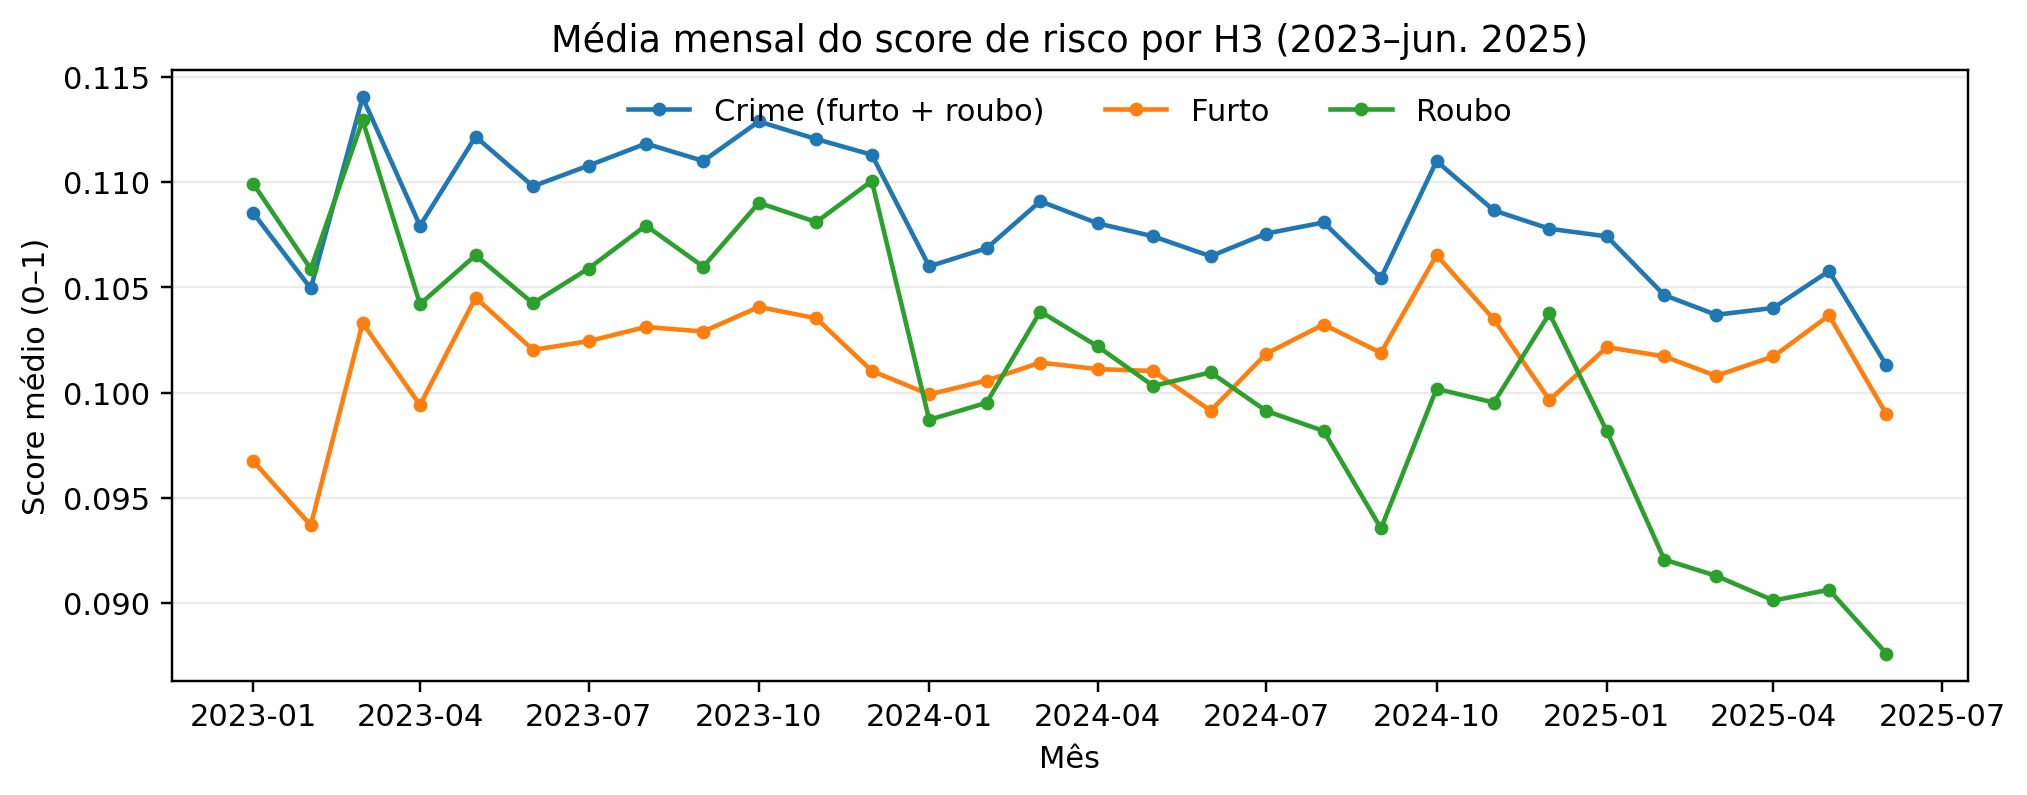
\includegraphics[width=.91\textwidth]{figuras/evolucao_mensal_risco.png}
\caption{Média mensal do score de risco entre as células H3 da RMSP. Cada alvo usa escala $K$ própria; as linhas devem ser comparadas ao longo do tempo dentro de cada alvo, não em altura entre alvos.}
\label{fig:risco_mensal}
\end{figure}

As associações bivariadas e a triagem de colinearidade também apontaram a força do histórico criminal. A média histórica da própria tipologia e as features sazonais aparecem entre as mais associadas aos alvos. Pares com correlação de Pearson absoluta de pelo menos 0,90 foram tratados como redundantes, priorizando uma representação; o VIF foi usado como diagnóstico complementar, com limiar de referência 5. Por exemplo, no conjunto candidato do crime, a feature de vizinhança absoluta foi removida por correlação de 0,916 com a média histórica própria; indicadores de casa, água, esgoto e coleta de lixo também eram altamente correlacionados. Essa triagem reduz redundância, mas não prova causalidade nem seleciona sozinha o melhor preditor. O desempenho fora do tempo é que orienta a escolha final do modelo.

\subsection{Validação temporal e teste reservado}

A Tabela~\ref{tab:validacao} mostra os modelos de menor RMSE médio na validação. Os três vencedores são globais e residuais: RF para crime e furto, GAM para roubo. O ganho sobre EWM3 foi pequeno para crime e especialmente para furto, e mais claro para roubo. Em todos os alvos, EWM3 superou a média histórica fixa, indicando que recência acrescenta informação à média estática da célula.

\begin{table}[!ht]
\centering
\caption{Melhor modelo por alvo na validação temporal (média de três folds)}
\label{tab:validacao}
\scriptsize
\renewcommand{\arraystretch}{1.15}
\begin{tabular}{l l r r r r r r}
\toprule
Alvo & Modelo & MAE & RMSE & $R^2$ & RMSE EWM3 & RMSE média fixa & Ganho vs EWM3 \\
\midrule
Crime & RF residual global & 0,0110 & 0,0201 & 0,9873 & 0,0204 & 0,0223 & 1,47\% \\
Furto & RF residual global & 0,0127 & 0,0232 & 0,9829 & 0,0233 & 0,0242 & 0,19\% \\
Roubo & GAM residual global & 0,0161 & 0,0294 & 0,9666 & 0,0304 & 0,0353 & 3,35\% \\
\bottomrule
\end{tabular}
\end{table}

O teste reservado confirma ganhos modestos, mas positivos, frente ao EWM3. Os vencedores da validação foram reajustados apenas com dados até junho de 2025 e mantiveram ganhos entre 2,06\% e 3,95\% no período posterior. A média histórica fixa apresentou erro maior que EWM3 e que os modelos escolhidos nos três alvos.

\begin{table}[!ht]
\centering
\caption{Resultado no teste reservado (jul./2025--jun./2026; 15.120 pares H3--mês por alvo)}
\label{tab:teste}
\scriptsize
\renewcommand{\arraystretch}{1.15}
\begin{tabular}{l l r r r r r}
\toprule
Alvo & Modelo selecionado & MAE & RMSE & $R^2$ & Ganho vs EWM3 & Ganho vs média fixa \\
\midrule
Crime & RF residual global & 0,0118 & 0,0225 & 0,9833 & 3,09\% & 24,24\% \\
Furto & RF residual global & 0,0134 & 0,0256 & 0,9790 & 2,06\% & 11,52\% \\
Roubo & GAM residual global & 0,0160 & 0,0293 & 0,9603 & 3,95\% & 38,45\% \\
\bottomrule
\end{tabular}
\end{table}

Os $R^2$ elevados refletem a capacidade de explicar variação do score no conjunto avaliado, mas não dispensam a comparação de erro com uma referência que já é forte. Para esse motivo, o ganho de RMSE sobre EWM3 é uma medida central: ela mostra a melhoria incremental efetivamente obtida. Também não se deve interpretar o score como probabilidade de vitimização; ele é uma transformação monotônica da contagem e serve como escala limitada de intensidade.

\subsection{O que a segmentação mudou}

A divisão entre grupos de alta e baixa atividade foi testada por alvo e definida somente com contagens de treino. Na maioria dos algoritmos, as estratégias com ajuste por grupo ou modelo híbrido apresentaram RMSE total próximo ao global e não produziram ganho estável. O Ridge direto teve erro muito alto, embora a segmentação o reduzisse; após a redução, continuou distante das melhores configurações. Além disso, a seleção por menor RMSE escolheu modelos globais para os três alvos. A evidência, portanto, não sustenta manter a segmentação como arquitetura principal neste experimento. Ela ainda poderia ser reconsiderada caso a métrica de interesse priorize especificamente o grupo de baixa atividade ou a captura de hotspots, o que é diferente do RMSE agregado usado aqui.

\subsection{Explicabilidade dos modelos finais}

A Figura~\ref{fig:importancia} resume a importância global das features nos ajustes finais. Para crime e furto, os sinais mais fortes na correção são a sazonalidade anual e os resíduos recentes; para roubo, destacam-se EWM3 e a média histórica logarítmica da própria célula. Isso indica que a contribuição adicional dos modelos continua ligada principalmente ao histórico criminal. Variáveis socioeconômicas e de moradia entram nos candidatos e podem contribuir, mas ficaram abaixo das principais features temporais nos modelos escolhidos.

\begin{figure}[!ht]
\centering
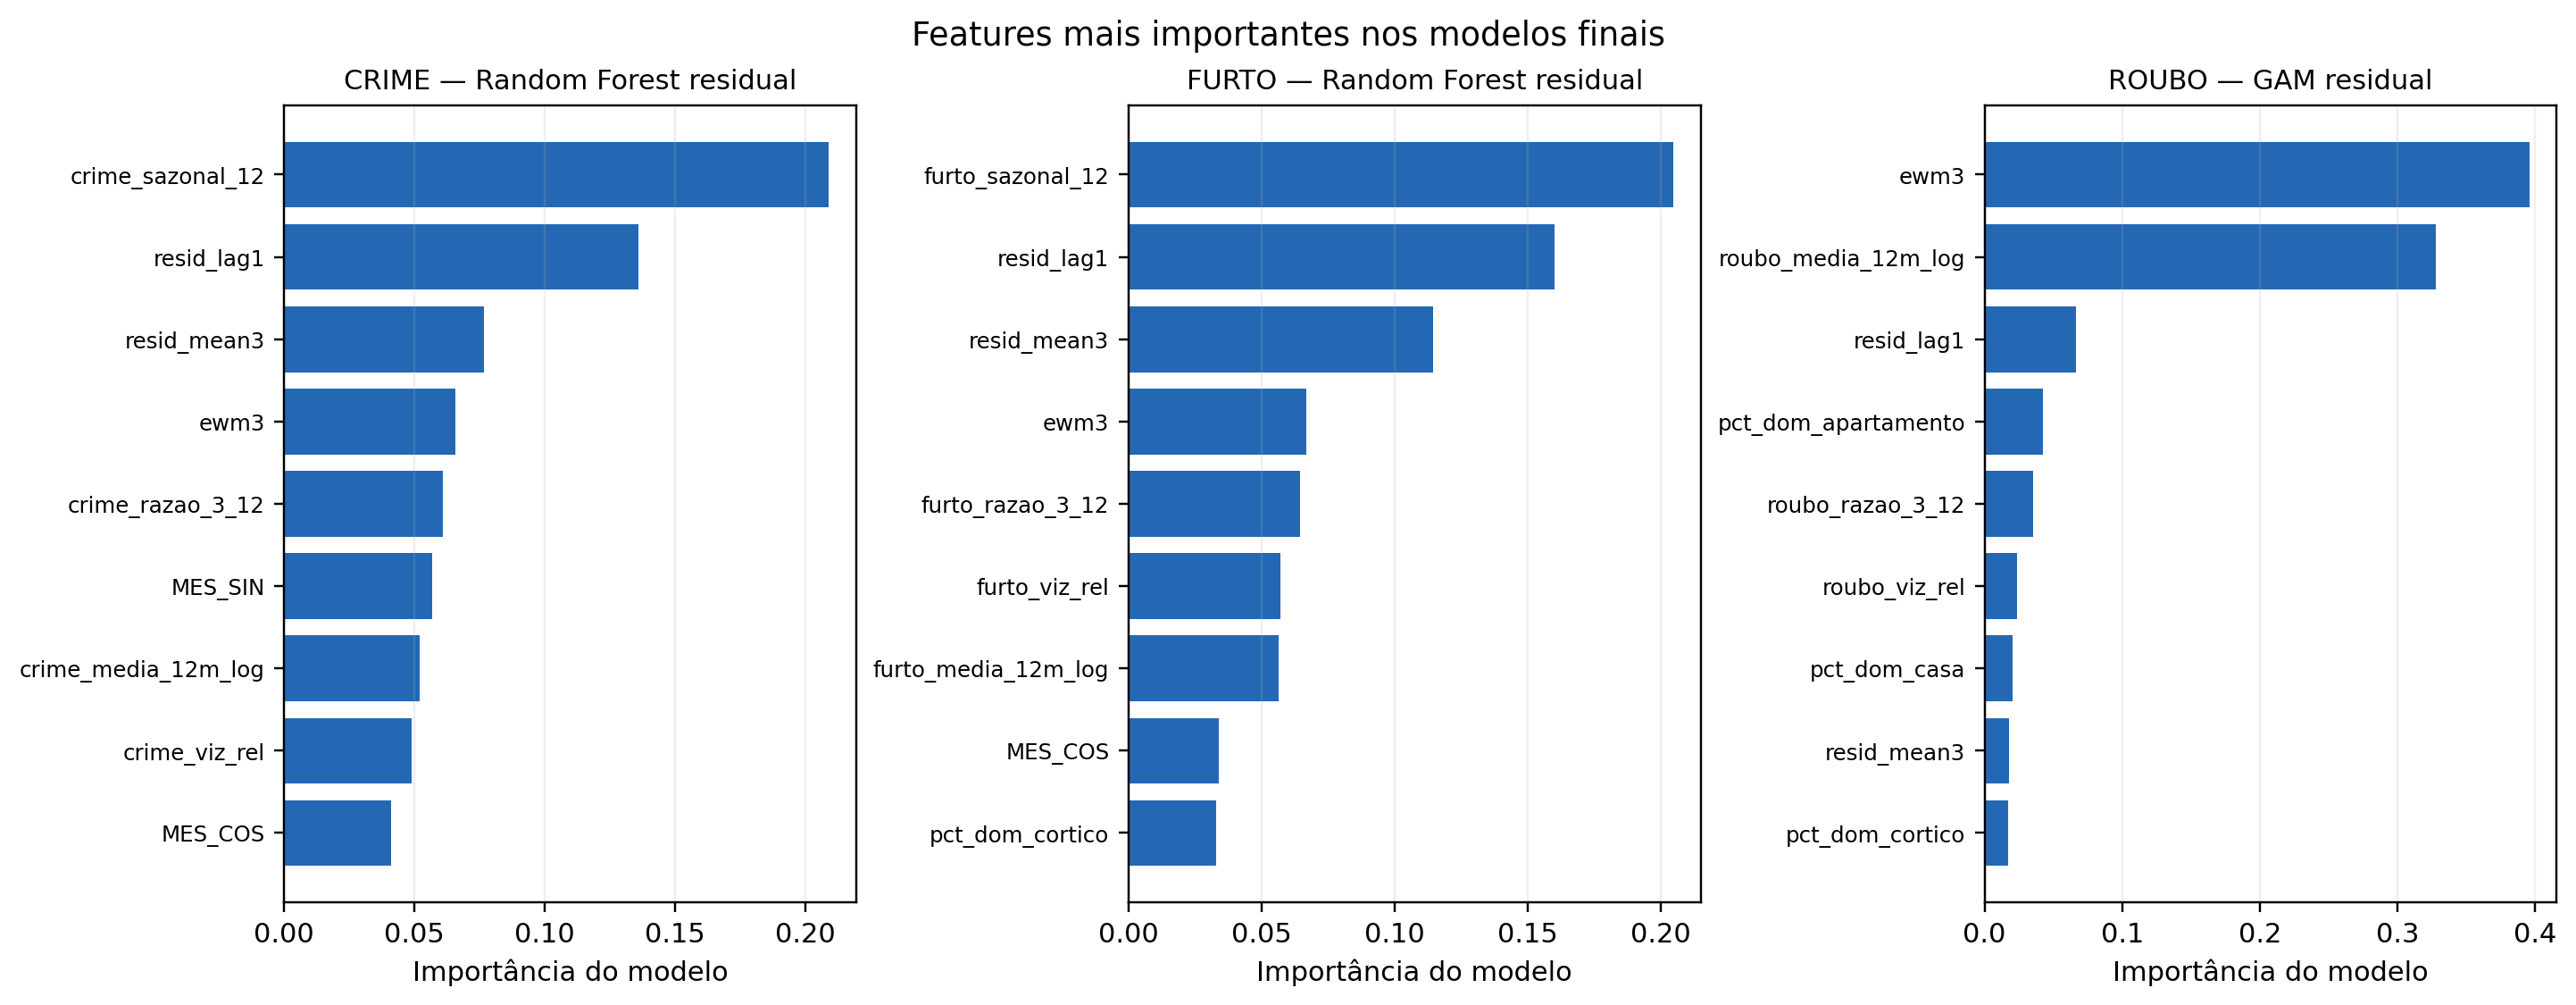
\includegraphics[width=.99\textwidth]{figuras/importancia_modelos_finais.png}
\caption{Features mais importantes nos modelos finais, calculadas no treino. As escalas são próprias do método de importância de cada modelo e não devem ser comparadas entre painéis. A importância corresponde à correção residual do EWM3.}
\label{fig:importancia}
\end{figure}

No RF, a importância por redução de impureza não indica direção nem efeito causal e pode repartir importância entre variáveis correlacionadas. No GAM, a barra agrega magnitudes de coeficientes spline, sem um único coeficiente linear por feature. Os testes do GAM residual apresentaram $p<0{,}0001$ tanto no Jarque--Bera quanto no Breusch--Pagan, apontando evidência contra normalidade e variância constante dos resíduos. A média do erro no teste foi $-0{,}0020$ (observado menos previsto), sinalizando pequena sobreprevisão média. Esses resultados recomendam cautela na inferência clássica sobre os efeitos suaves, mas não anulam a avaliação preditiva no teste reservado.

\subsection{Por que é difícil superar o EWM3?}

A evidência aponta para uma tarefa de ganho incremental. Primeiro, o EWM3 atualiza a estimativa com os próprios resultados recentes da célula e já supera a média histórica fixa, que ignora mudanças de nível. Segundo, o score apresenta grande proporção de zeros e forte concentração em uma minoria de células; esse ruído e a heterogeneidade dificultam estimar a variação mensal. Terceiro, as features socioeconômicas são de 2022 e relativamente estáticas, enquanto a correção desejada é mês a mês. Por fim, as features de vizinhança trazem informação espacial, mas não foram suficientes para tornar a segmentação alto/baixo consistentemente superior.

A comparação residual testa diretamente se os dados disponíveis explicam o que o EWM3 erra. Os ganhos modestos na validação e no teste mostram que há informação adicional, mas ela é pequena frente à persistência já capturada pelo histórico suavizado. O fato de o ganho se repetir no teste reservado é promissor, embora não deva ser extrapolado sem nova avaliação temporal quando novas observações estiverem disponíveis.

\subsection{Interface de mapa -- espaço reservado}

\textit{[Seção reservada para descrever a interface cartográfica, as camadas de risco, os filtros temporais e a forma de consulta por célula H3. A interface ainda não está implementada e nenhum resultado cartográfico é apresentado nesta versão.]}

\section{Conclusão}

O estudo construiu uma série mensal por H3 para a RMSP, integrou contexto socioeconômico de 2022 e comparou modelos contra média histórica e EWM3 sob validação temporal. As correções residuais globais foram as melhores configurações: RF para crime e furto, e GAM para roubo. No teste reservado, reduziram o RMSE do EWM3 entre 2,06\% e 3,95\%; a divisão alto/baixo não trouxe ganhos consistentes. A análise de importância mostrou predominância de features temporais e históricas, enquanto os diagnósticos do GAM limitam a interpretação inferencial de seus efeitos. Como limitações, a avaliação é rolling de um mês, o score não é probabilidade e o contexto socioeconômico é estático. A próxima etapa é desenvolver a interface de mapa e avaliar sua utilidade para priorização territorial, sem confundir visualização com evidência de melhora preditiva.

\bibliographystyle{plain}
\bibliography{referencias}
\end{document}
